

%================================================================
%\chapter{Computational Neuroscience}\label{chap:compneuro}
%================================================================


%================================================================
\chapter{Neuroscientific Models}\label{chap:compneuro}
%================================================================


%================================================================
\section{The Hodgkin-Huxley Model}
%================================================================


%================================================================
\section{The Brunel Network Model}
%================================================================

\subsection{Leaky integrate and fire neurons}

\subsection{Spike Train Statistics}

Spikes are events characterized by their firing time $t^{(f)}$, where $f=1, 2, ...$ labels a spike by the spike count. We define the spike train of a neuron $i$ as the sequence of firing times: 

\begin{equation}
    S_i(t) = \sum_f \delta \left(t - t_i^{(f)} \right),
\end{equation}

where $\delta(x)$ is the Dirac $\delta$ function with $\delta(x)=0$ for $x \neq 0$ and $\int_{-\infty}^\infty \delta (x) \dd{x} = 1$. Thus, spikes are reduced to points in time. 

\textbf{Mean firing rate in thesis}

We use a time and population averaged firing rate. 

The time averaged firing rate of a single spike train is calculated as the number of spikes in the spike train in the time interval $T = [t_\mathrm{start}, t_\mathrm{stop}]$ divided by the time interval $T$. 

The population average is subsequently calculated by averaging over all the $N_\mathrm{rec}$ recorded neurons, resulting in the mean firing rate.  

Formally, the above procedure can be denoted by: 

\begin{equation}
    \bar{\eta} = \frac{1}{N_\mathrm{rec} \left(T_\mathrm{sim} - T_\mathrm{transient}\right)} \int_{T_\mathrm{transient}}^{T_\mathrm{sim}} \sum_i \sum_f \delta \left(t - t_i^{(f)} \right) \dd{t}
\end{equation}

Time resolved firing rate: 

Histogram: Binned the spike trains in bins of $\Delta t = 10$ ms.

\begin{equation}
    \eta (t) = \frac{1}{N_\mathrm{rec} \Delta t} \int_{t}^{t + \Delta t} \sum_i \sum_f \delta \left(t - t_i^{(f)} \right) \dd{t}
\end{equation}

\subsection{Recurrent network of LIF}


\autoref{fig:brunel_states} illustrates an example of each of the states of the Brunel network. For each state, the figure shows the firing times (rasters) of 20 randomly chosen neurons, the temporal evolution of the activity of the system (time resolved firing rate computed in bins of 10 ms) together with the mean firing rate (horizontal axis line), and the correlation coefficient matrix of the recorded neurons.


\begin{figure}[H]
    \centering
    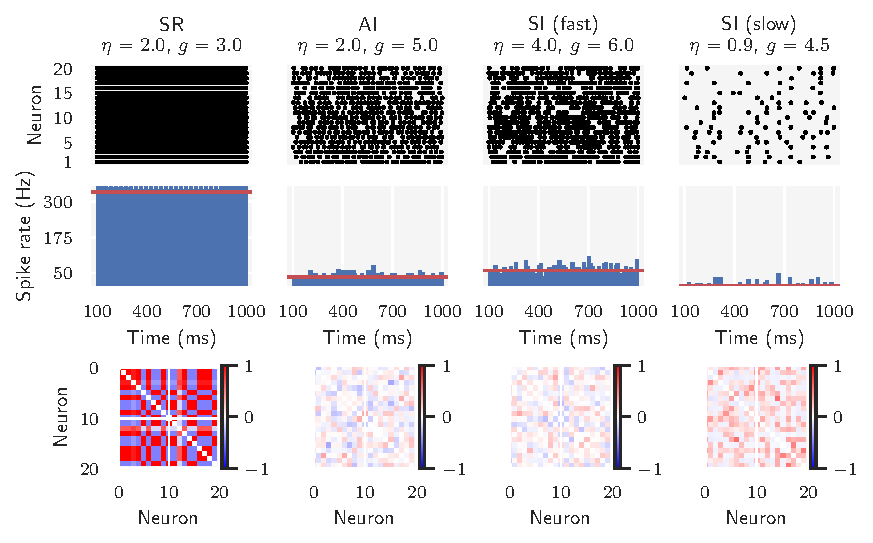
\includegraphics[scale=1.0]{brunel_states}
    \caption{Simulation of a network of $N_\mathrm{E}=10,000$ excitatory and $N_\mathrm{I} = 2,500$ inhibitory neurons with connection probability $\epsilon = 0.1$, which corresponds to a network where each neuron has $C_\mathrm{E}=1,000$ and $C_\mathrm{I}=250$ randomly selected connections to excitatory and inhibitory neurons, respectively. Each spike causes, after a delay of $D=1.5$ ms (synaptic delay), a voltage jump of $J_E = 0.1$ mV (amplitude of excitatory synaptic currents). The distance from equilibrium potential to firing threshold is $V_\mathrm{th} = 20$ mV; absolute refractory period $\tau_\mathrm{rp} = 2$ ms; membrane time constant $\tau_\mathrm{m}=20$ ms; membrane capacitance $C_m = 1$ pF. The network is simulated for $T_\mathrm{sim} = 1,000$ ms, and we record the output from $N_\mathrm{rec} = 20$ excitatory neurons. To avoid transient effects, we start recording after $T_\mathrm{transient} = 100$ ms. 
    }
    \label{fig:brunel_states}
\end{figure}


SR: Almost fully synchronized network, neurons firing regularly at high rates.

AI: Stationary global activity (see text), irregularly firing neurons

SI fast: Fast oscillation of the global activity, neurons firing irregularly at a rate that is lower than the global frequency

SI slow: Slow oscillation of the global activity, neurons firing irregularly at very low rates



%================================================================
\section{Notes}
%================================================================

%================================================================
%\chapter{Computational Neuroscience}\label{chap:compneuro}
%================================================================

From Theoretical neuroscience : computational and mathematical modeling of neural
systems / Peter Dayan and L.F. Abbott.


Computational neuroscience is an approach to understanding the information content of neural signals by modeling the nervous system at many different structural scales, including the biophysical, the circuit, and the systems levels. Computer simulations of neurons and neural networks are complementary to traditional techniques in neuroscience. This book series welcomes contributions that link theoretical studies with experimental approaches to understanding information processing in the nervous system. Areas and topics of particular interest include biophysical mechanisms for computation in neurons, computer simulations of neural circuits, models of learning, representation of sensory information in neural networks, systems models of sensory-motor integration, and computational analysis of problems in biological sensing, motor control, and perception.

--

Theoretical analysis and computational modeling are important tools for characterizing what nervous systems do, determining how they function, and understanding why they operate in particular ways. Neuroscience encompasses approaches ranging from molecular and cellular studies to human psychophysics and psychology. Theoretical neuroscience encourages crosstalk among these subdisciplines by constructing compact representations of what has been learned, building bridges between different levels of description, and identifying unifying concepts and principles. In this book, we present the basic methods used for these purposes and discuss examples in which theoretical approaches have yielded insight into nervous system function.

The questions what, how, and why are addressed by descriptive, mechanistic, and interpretive models, each of which we discuss in the following chapters. Descriptive models summarize large amounts of experimental data compactly yet accurately, thereby characterizing what neurons and neural circuits do. These models may be based loosely on biophysical, anatomical, and physiological findings, but their primary purpose is to describe phenomena, not to explain them. Mechanistic models, on the other hand, address the question of how nervous systems operate on the basis of known anatomy, physiology, and circuitry. Such models often form a bridge between descriptive models couched at different levels. Interpretive models use computational and information-theoretic principles to explore the behavioral and cognitive significance of various aspects of nervous system function, addressing the question of why nervous systems operate as they do.

It is often difficult to identify the appropriate level of modeling for a particular problem. A frequent mistake is to assume that a more detailed model is necessarily superior. Because models act as bridges between levels of understanding, they must be detailed enough to make contact with the lower level yet simple enough to provide clear results at the higher level.

\section{Modeling Electrical Activity in Neurons}

\subsubsection{The electric force on ions}

As ions are electrically charged they exert forces on and experience forces from other ions. The force acting on an ion is proportional to the ion’s charge, $q$. The \textit{electric field} at any point in space is defined as the force experienced by an object with a unit of positive charge. A positively charged ion in an electric field experiences a force acting in the direction of the electric field; a negatively charged ion experiences a force acting in exactly the opposite direction to the electric field. At any point in an electric field a charge has an \textit{electrical potential energy}. The difference in the potential energy per unit charge between any two points in the field is called the \textit{potential difference}, denoted $V$ and measured in volts.

\subsubsection{Cell membrane is a capacitor} 

That the cell membrane is a capacitor means there is a voltage difference $V$ across it, accompanied by equal positive ($Q+$) and negative ($Q-$) charges on each side of the neuron. 

A capacitor consists of two conductors separated by a non-conductive region. The non-conductive region can either be a vacuum or an electrical insulator material known as a dielectric. From Coulomb's law a charge on one conductor will exert a force on the charge carriers within the other conductor, attracting opposite polarity charge and repelling like polarity charges, thus an opposite polarity charge will be induced on the surface of the other conductor. The conductors thus hold equal and opposite charges on their facing surfaces, and the dielectric develops an electric field.

The strength of the electric field set up through the separation of ions between the plates of the capacitor is proportional to the magnitude of the excess charge $q$ on the plates. As the potential difference is proportional to the electric field, this means that the charge is proportional to the potential difference. The constant of proportionality is called the **capacitance** and is measured in **farads**. It is usually denoted by $C$ and indicates how much charge can be stored on a particular capacitor for a given potential difference across it:

$$ q = C V $$


%================================================================
\subsection{The Hodgkin-Huxley Model}\label{sec:hh}
%================================================================ 

\url{http://www.sci.utah.edu/~macleod/bioen/be6003/notes/W09-encyc_human_brain_00.pdf}

\url{http://www.inf.ed.ac.uk/teaching/courses/nc/NClab2.pdf}

In their Nobel prize winning work [cite], Hodgkin and Huxley developed a model for the initiation and propagation of action potentials in the squid giant axon. 

\url{https://hodgkin-huxley-tutorial.readthedocs.io/en/latest/}

Reference to equations in original paper: 

\url{https://github.com/swharden/HHSharp/blob/master/src/HHSharp/HHModel.cs}

Describes how the membrane potential $V_m$, that is, the voltage across a membrane with capacitance $C$, responds to an input current $I$.


\url{https://www.ncbi.nlm.nih.gov/pmc/articles/PMC3219615/}
There are several sources to noise in cellular dynamics. [article] provides an excellent review of stochastic versions of the HH equations. [To model channel noise within a differential equation framework of the general form above, we seek ways of introducing fluctuations into this deterministic system.] Current noise, subunit noise, conductance noise. We only look at current noise in this thesis

Gaussian white noise (GWN) is a stationary and ergodic random process with zero mean that is defined by the following fundamental property: any two values of GWN are statistically independent now matter how close they are in time. 

Although the mathematical properties of GWN have been studied extensively and utilized in many fields, the ideal GWN signal is not physically realizable because it has infinite variance by definition (recall that the variance of a stationary zero-mean random signal is equal to the value of its autocorrelation function at zero lag).


%================================================================ 
\subsubsection{Channel Kinetics}
%================================================================ 

\url{https://pubmed.ncbi.nlm.nih.gov/8845165/}

In the standard Hodgkin-Huxley model. the primary contribution to the initiation and propagation of single action potentials is made by the fast \Na channel. A single noninactivating, voltage-dependent \K current provides spike repolarization. 

The \Na current is calculated using the standard ohmic relation

\begin{equation*}
    I_{Na} = \bar{g}_{Na} m^3 h \qty(V_m - E_{Na}),
\end{equation*}

where $I_{Na}$ is the \Na current, $V_m$ is the membrane potential, $E_{Na}$ is the equilibrium potential for \Na (assumed to be $+50 mV$), and $m$ and $h$ are the activation and inactivation state variables, respectively. The variable $m$ ranges from $0$ (not activated) to $1$ (fully activated), and $h$ ranges from $0$ (fully inactivated) to $1$ (no inactivation). The maximal conductance is the product $\bar{g}_{Na} = \gamma_{Na} \rho_{Na}$ where $\gamma_{Na}$ is the single channel conductance and $\rho_{Na}$ is the channel density. 

$I_{Na}$ activation is described by the usual first order kinetic reaction, $\text{open} \xrightleftharpoons[]{} \text{closed}$, which yields steady-state value $m_\infty$ and time constant $\tau_m$ given by 

\begin{align*}
    m_\infty &= \frac{\alpha}{\alpha + \beta}, 
    \\ 
    \tau_m &= \frac{1}{\alpha + \beta},
\end{align*}

where $\alpha$ and $\beta$, the forward (opening) and backward (closing) reaction rates, respectively, are functions of the local membrane potential. Specifically, 

\begin{align*}
    \alpha \qty(V_m) &= \frac{A \qty(V_m - V_{1/2})}{1 - \mathrm{e}^{- \qty(V_m - V_{1/2})/k}},
    \\
    \beta \qty(V_m) &= \frac{-A \qty(V_m - V_{1/2})}{1 - \mathrm{e}^{- \qty(V_m - V_{1/2})/k}},
\end{align*}

where $A$ is a rate constant, $V_{1/2}$ is the half-activation voltage, and $k$ determines the slope of the activation curve. 

(See Table 1 and 2 in article)


%================================================================ 
\subsubsection{HH in neural simulation software}
%================================================================ 

\url{http://nelson.beckman.illinois.edu/courses/physl317/part1/Lec3_HHsection.pdf}

In neural simulation software packages, the rate constants in HH-style models are often parameterized using a generic functional form:

\begin{equation*}
    \alpha (V) = \frac{A + BV}{C + H \exp \qty(\frac{V+D}{F})}
\end{equation*}

In general, this functional form may require up to six parameters $(A, B, C, D, F, H)$ to fully specify the rate equation. However, in many cases adequate fits to the data can be obtained using far fewer parameters. Fortunately, Eq. 29 is flexible enough that it can be transformed into simpler functional forms by setting certain parameters to either 0 or 1. For example, if the voltage clamp data can be adequately fit by an exponential function over the relevant range of voltages, then setting $B=0$, $C=0$, $D=0$ and $H=1$ in Eq. 29, results in a simple exponential form,
$\alpha(V) = A \exp(-V / F)$ , with just two free parameters ($A$ and $F$) to be fit to the data. Similarly, setting B=0, C=1 and H=1 gives a sigmoidal function with three free parameters ($A$, $D$, and $F$).

One other technical note is that certain function forms can become indeterminate at
certain voltage values. For example, the expression for $(V)$ an in Eq. 23 evaluates to the indeterminate form $0/0$ at $V=10$. The solution to this problem is to apply L’Hospital’s rule, which states that if $f(x)$ and $g(x)$ approach $0$ as $x$ approaches $a$, and $f'(x)/ g'( x)$ approaches $L$ as $x$ approaches $a$, then the ratio $f (x)/ g( x)$ approaches $L$ as well. Using this rule, it can be shown
that $\alpha_n (10) = 0.1$. When implementing HH-style rate functions in computer code, care must be taken to handle such cases appropriately.

Stability

\url{https://timvieira.github.io/blog/post/2014/02/11/exp-normalize-trick/}

\url{https://gregorygundersen.com/blog/2020/02/09/log-sum-exp/}


Suggestions for how to diagnose the problems you may encounter:

\begin{enumerate}
    \item Start small and add complexities incrementally, testing at every step. It doesn't matter how smart you are, how facile you may be with programming, or how hard you work -- frustration and debugging nightmares are guaranteed if you try to do it all in one pass.
    \item Use modlunit to verify consistency of units. modlunit will also pick up many programming errors.
    \item Make sure that all ionic conductances have the desired properties. Plot the alphas and betas as functions of membrane potential. Do "voltage clamp" experiments on a single compartment model and plot the time course of m, h, n, gna, gk, ina, and ik. Also make sure that leak current has the correct voltage dependence.
    \item Use L'hospital's rule to avoid rate constant formulas that become indeterminate (0/0) (alphan and alpham). Look at hh.mod for an example. \url{https://github.com/neuronsimulator/nrn/blob/master/src/nrnoc/hh.mod}
\end{enumerate}


%================================================================ 
\subsubsection{Derivations}
%================================================================ 

In HH paper (1952): 

\begin{equation*}
    \alpha_n = 0.01 \cdot \frac{V+10}{\exp \qty(\frac{V+10}{10})-1}
\end{equation*}

Let $A=0.01$, $x=V+10$, and $y=10$, such that

\begin{equation*}
    \alpha_n = A \cdot \frac{x}{\exp \qty(\frac{x}{y})-1}
\end{equation*}

An alternative form for the above equation can be found by: 

\begin{equation*}
    \alpha_n = A \cdot \frac{x}{\exp \qty(\frac{x}{y})-1} \cdot \frac{(-1)}{(-1)} = A \cdot \frac{-x}{1-\exp \qty(\frac{x}{y})} 
\end{equation*}

Changing $x=V+10 \rightarrow x = - (V+55)$ and inserting in the last equation gives:

\begin{equation*}
    \alpha_n = 0.01 \cdot \frac{V+55}{1 - \exp \qty(-\frac{V+55}{10})},
\end{equation*}

which is the form found in Sterratt.

%================================================================ 
\subsubsection{Deriving Vtrap}
%================================================================ 

The general form for this equation is:

vtrap = x/(exp(x/y) - 1)

however as can be easily seen if x/y is 0, or close to zero, then the denominator of the given equation is really small or zero, leading to and infinite or very large output. To get around this when x/y is really small the output is given as:

vtrap = y*(1 - x/y/2) or as I prefer y - x/2

---

The rate equations becomes indeterminate at certain membrane potentials, for instance, $\alpha_n (-55) = 0 / 0$. 


A Taylor Series is an expansion of some function into an infinite sum of terms,

The Taylor series of

We can use the first few terms of a Taylor Series to get an approximate value for a function.


A Taylor series is a series expansion of a function about a point. A one-dimensional Taylor series is an expansion of a real function f(x) about a point x=a is given by

%%%

Traps for 0 in denominator of rate eqns. 

Alternative func name: SafeExp


The vtrap function was correct in its original form, which approximated x/(exp(x/y) - 1) by a straight line segment with the appropriate slope in the near neighborhood of |x/y|==0. You just replaced that approximation with something that will cause a discontinuity of a voltage-dependent gating parameter when v lands within a narrow band centered on x/y==0. Will that cause problems for you or anyone who reuses your code in the future? Maybe, if adaptive integration is used--the adaptive integrators require voltage-dependent parameters to be continuous functions of membrane potential, but the occasional violation of continuity may not always cause a noticeable problem.


Remember, you're dealing with a computational representation of physical system which is continuous in space and time (when viewed at the scale of microns and microseconds). The continuous system is described by a PDE, but you're using numerical solution of a set of ODEs to approximate the solution to the PDE, and that requires discretizing both space and time. Spatial discretization approximates the PDE by a family of ODEs, where each ODE describes the time course of state variables at a different point in space. Accuracy of the entire solution depends not only on dt, the interval at which you sample time, but also on dx, the interval at which you sample space. Make dt very small, and you will expose spatial errors, which become predominant at short times.

avoid numerical under flow

To help get you started, here's a little background on vtrap and some hints:

HH-style model rate equations often contain expressions that are equivalent to

$$x / (exp(x/y) - 1)$$

As $x/y -> 0$, the numerator and denominator $-> 0$, which can cause problems.
This can be avoided by noting that, as $x/y -> 0$,

$$exp(x/y) - 1 = 1 + x/y + ((x/y)^2)/2 + . . . - 1$$

approaches

$$x/y + (x^2)/((y^2)*2)$$

so

$$x / (exp(x/y) - 1)$$

approaches

$$x / (x/y + (x^2)/((y^2)*2)) = y / (1 + x/(2*y))$$

which is closely approximated by

$$y * (1 - x/(2*y))$$

when $x/(2*y) << 1$.

%================================================================ 
\subsubsection{Stiffness}
%================================================================ 

Lambert (1992) defines stiffness as follows:
If a numerical method [. . . ] applied to a system
with any initial conditions, is forced to use in a
certain interval of integration a steplength which is
excessively small in relation to the smoothness of the
exact solution in that interval, then the system is said
to be stiff in that interval.
A typical case of stiffness is for example, when different parts of
the solution of a system of equations decays on different time
scales.
This usually comes from very different scales inherent to the
ODE. These scales will reflect in the parameters of the equations,
i.e., the range of constants occurring in the equations of the
systems. Therefore the stiffness of a system always depends not
only on the mathematical form of the equations but heavily on
the magnitude of the constants occurring in them.
In principle it is possible to solve stiff equations with explicit
methods, but this comes at the expense of a very small step size
when using an adaptive step size algorithm and trying to achieve
a certain accuracy. This in turn leads to high computational
costs. For non-adaptive step size algorithms it leads to plain
wrong results without the user knowing, since the algorithm
still terminates, but with large error. Moreover, as the limited
machine precision on a digital computer constitutes a lower
bound for the step size, explicit methods usually become unstable
when applied to stiff problems.
Implicit methods, on the other hand, do not use previous
values to calculate the solution at the next grid point, but only
employ them implicitly in the form of the solution of a system of
equations. This makes implicit methods computationally much
more costly, but usually allows a larger step size to be chosen,
thus avoiding stability problems (Strehmel and Weiner, 1995).
In order to detect whether an explicit or implicit method is
better suited for a given ODE we devise the following testing
strategy.

Moreover, as the limited
machine precision on a digital computer constitutes a lower
bound for the step size, explicit methods usually become unstable
when applied to stiff problems.


%================================================================ 
\subsubsection{Models of Active Ion Channels}
%================================================================

Sterratt 

5.3.2 

HH succeeded in isolating three currents with distinct kinetics (the sodium, potassium delayed rectifier and leak currents).


Thermodynamical equations 

Excerpt from Action Potentials - HH Eq, FN eq:

The Hodgkin-Huxley model proved to be very accurate and useful in further research into action potentials. However, the formula was rather complicated and \textbf{relied heavily on empirical equations to fit the data}. 

Thermodynamic models - principled way to model rate equations, i.e. is based on the biophysical theory of channels. 

sec 5.4.2 Thermodynamic models

In Box 5.2 there are effectively five different forms of function to fit the dependence on voltage of the rate coefficients $\alpha_m (V)$, $\beta_m (V)$ and so on: three for the HH sodium and potassium channels and two for the A-type potassium channel. All these forms satisfy the critical requirement of fitting the data well. However, it is desirable to base the form of these functions as much as possible on the biophysical theory of channels, \textbf{since fitting to the most principled function is likely to minimise errors due to fitting}.

\section{The Integrate- and Fire Neuron Model}

Providing an answer to the question whether IF models provide an adequate simplification of biophysically based models is therefore important in the quest for a better un- derstanding of the nature of the neural code.

%================================================================ 
\section{Network Models}
%================================================================

\url{https://www.ncbi.nlm.nih.gov/pmc/articles/PMC6193674/pdf/bhw237.pdf}

Modeling large-scale neural-network dynamics with individual spiking neurons is challenging due to the memory required to represent the large number of synapses. With current technology and using the largest supercomputers available today, simulations of neural networks comprising up to 109 neurons and 1013 synapses (roughly corresponding to the size of a cat brain) are feasible for simplified model neurons (Diesmann 2013; Kunkel et al. 2014). Typically, these simplified models
neglect the spatial aspects of neuronal morphologies and describe neurons as points in space (point-neuron models).
Despite their simplicity, point-neuron-network models explain
a variety of salient features of neural activity observed in vivo,
such as spike-train irregularity (Softky and Koch 1993; van
Vreeswijk and Sompolinsky 1996; Amit and Brunel 1997;
Shadlen and Newsome 1998), membrane-potential fluctuations
(Destexhe and Paré 1999), asynchronous firing (Ecker et al. 2010;
Renart et al. 2010; Ostojic 2014), correlations in neural activity
(Gentet et al. 2010; Okun and Lampl 2008; Helias et al. 2013),
self-sustained activity (Ohbayashi et al. 2003; Kriener et al.
2014), and realistic firing rates across laminar cortical populations (Potjans and Diesmann 2014). Point-neuron networks are
amenable to mathematical analysis (see, e.g., Brunel 2000; Deco
et al. 2008; Tetzlaff et al. 2012; Helias et al. 2013; de Kamps
2013; Schuecker et al. 2015; Bos et al. 2016) and can be efficiently evaluated numerically (Brette et al. 2007; Plesser et al.
2007; Helias et al. 2012; Kunkel et al. 2014). The mechanisms
governing networks of biophysically detailed multicompartment model neurons, in contrast, are less accessible to analysis
and these models are more prone to overfitting. Existing multicompartment neuron network models accounting for realistic
cell morphologies are restricted to sizes of $\sim104
–105$ neurons
(Hines et al. 2008; Reimann et al. 2013; Migliore et al. 2014;
Markram et al. 2015). Large-scale models are, however, necessary to include contributions to the LFP from distant populations in situations where the spatial reach of the LFP is known
to be large (Lindén et al. 2011; Łe¸ski et al. 2013). 

Although point-neuron networks capture many features of
in vivo spiking activity, they fail to predict extracellular potentials that result from transmembrane currents distributed
across the cell surface. According to Kirchhoff’s law of current conservation, the sum of all transmembrane currents, including all ionic and capacitive currents, must be zero for each neuron. In a point-neuron model, all transmembrane currents are
collapsed in a single point in space. The net transmembrane
current, and hence the extracellular potential, therefore
vanishes. Only the spatial separation between current sinks
and sources leads to a nonzero extracellular potential
(Pettersen et al. 2012; Einevoll et al. 2013). A priori, the prediction of extracellular potentials, therefore, requires spatially
extended neuron models accounting for the spatial distribution
of transmembrane currents, commonly handled using multicompartment neuron models (De Schutter and Van Geit 2009).
Note that the principle of current conservation implies a current sum rule for multicompartment neuron models as well:
the sum of all single-cell transmembrane currents remains
zero, also across neuron populations and the whole column. In
several previous studies (Bazhenov et al. 2001; Hill and Tononi
2005; Ursino and La Cara 2006; Mazzoni et al. 2008; 2010; 2011),
the activity of point-neuron networks (e.g., population firing
rates, synaptic currents and membrane potentials) has nevertheless been used as a proxy for the LFP when comparing with
experiments. In a recent study comparing different candidate
proxies, it was found that a suitably chosen sum of synaptic
currents could provide a good LFP proxy, but only for the case
when the LFP is generated from transmembrane currents of a
single population of pyramidal neurons (Mazzoni et al. 2015). In
cortex, however, several populations in general contribute to
the LFP, and there are spatial cancellation effects when positive
LFP contributions from one population overlap in space with
negative LFP contributions from other populations. This effect
cannot be accounted for by a simple LFP proxy.

In this article, we present a hybrid modeling scheme that
combines the simplicity and efficiency of point-neuron network
models and the biophysical principles underlying LFP generation captured by multicompartment neuron models with anatomically reconstructed morphologies. The scheme allows for
arbitrary numbers of LFP-contributing populations, and directly
incorporates spatial cancellation effects. Furthermore, the spatially extended LFP-generating neurons assure that effects from
intrinsic dendritic filtering of synaptic inputs are included in
the predicted LFP (Lindén et al. 2010). The scheme assumes
that the spiking activity of the neural network (Fig. 1B) generating the synaptic input reflected in the LFP is well described by a
point-neuron network model (Fig. 1A). The network spiking
activity serves as synaptic input to a population of mutually
unconnected multicompartment model neurons with realistic
morphologies positioned in 3-dimensional (3D) space (Fig. 1C)
and is thereby translated into a distribution of transmembrane
currents and, hence, an LFP (Fig. 1D). Thus each multicompartment model neuron has its equivalent in the point-neuron network and receives input spikes from the same presynaptic
neurons as this point-neuron equivalent.

In the proposed hybrid modeling scheme, the LFP stems from
the presynaptic spiking activity, but does not affect the spikegeneration dynamics. Thus, the modeling of the spike trains and
the LFP generation are separated so that the effects of the spatial
and electrophysiological properties of the postsynaptic (multicompartment) neurons on the LFP can be investigated independently of the spike-generation dynamics. Due to the linearity of
Maxwell’s equations and volume conduction theory linking
transmembrane currents to extracellular potentials (Pettersen
et al. 2012; Einevoll et al. 2013), the compound LFP results from
the linear superposition of all single-cell LFPs generated by the
collection of neurons in the multicompartment model neuron population (Einevoll et al. 2013). Note that this linear superposition principle applies even for nonlinear cell dynamics (e.g.,
nonlinear synaptic integration, action-potential generation and
active conductances) as in Reimann et al. 2013. As ephaptic
interactions (Anastassiou et al. 2011) are neglected, the LFP contribution from each multicompartment model neuron can be
treated independently from the others. The computational
hybrid LFP scheme proposed here exploits the methodological
and conceptual advantages due to the independence of the contributions to the LFP from each multicompartment model neuron: the evaluation of the LFPs becomes “embarrassingly
parallel” (see Foster 1995) and simulations of the multicompartment model neuron dynamics can be easily distributed in parallel across many compute units (i.e., CPUs). Although tailored
toward use on high-performance computing facilities, the hybrid
simulation can in principle be run on a single laptop.

The hybrid scheme predicts spatially and temporally
resolved neural activity at various scales: spikes, synaptic currents, membrane potentials, current-source densities (CSD, see
e.g., Nicholson and Freeman 1975; Pettersen et al. 2006; 2008),
and LFPs. It therefore allows for investigation of relationships
between different measures of neural activity. Thus, although
point-neuron networks until now only have connected to
in vivo experiments via measurement of spikes, single-neuron
membrane potentials and currents, the present hybrid scheme
allows for comparison of model predictions also with measured
LFPs (and associated CSDs).

\section{Spike Train Statistics}
In the next few sections, we introduce some important concepts commonly used for the statistical description of neuronal spike trains. Central notions will be the interspike interval distribution, (Section 7.3), the noise spectrum (Section 7.4), but most importantly the concept of ‘firing rate’ which we discuss first.

A spike train is the sequence of neuronal firing timings, where a spike refers to the firing of an action potential. The temporal pattern of a spike train encodes information in various ways. Besides firing rates, the temporal pattern of spike timings also carries important information about brain functions. 

See: Dayan and Abbott, Ch. 1

\url{https://www.frontiersin.org/articles/10.3389/fncom.2019.00082/full}

\url{https://neuronaldynamics.epfl.ch/online/Ch7.S1.html}

The toolbox Elephant (RRID:SCR\_003833) provides the foundation to extract well-defined and comparable features of the network dynamics. 

The frequency by which neurons generate spikes (action potentials) is commonly considered as a basic form of information transfer within the neuronal system (Adrian and Zotterman, 1926; Perkel and Bullock, 1968). This “frequency code” is often quantified by the number of spikes within an appropriately set time window. The length of the window is limited by the requirement of stable conditions on one side, and by aiming at reproducible results on the other side. The natural conditions typically vary rapidly, but even if kept constant by an experimenter, there are other reasons, like spiking adaptation (Benda and Herz, 2003), which restrict the duration of the observation time window. All these constrains create difficulties for the statistical inference based on the firing rate, and many sophisticated methods to overcome them have been developed (Nawrot et al., 1999; Dayan and Abbott, 2001; Cunningham et al., 2009; Benedetto et al., 2015; Kostal et al., 2018; Tomar, 2019).

\url{https://www.frontiersin.org/articles/10.3389/fncom.2020.569049/full}

\subsection{Brunel}

Uncertainpy paper:
\url{https://www.frontiersin.org/articles/10.3389/fninf.2018.00049/full}

Brunel paper: 
\url{https://link.springer.com/content/pdf/10.1023/A:1008925309027.pdf} 

Neurodynamics: 
\url{https://neuronaldynamics.epfl.ch/online/Ch13.S4.html}
\url{https://neuronaldynamics.epfl.ch/online/Ch7.S2.html}
\url{https://neuronaldynamics.epfl.ch/online/Ch1.S3.html}